% プロコン 2026 展示ポスター（A0 縦）
% 版面は A1 で組み、poster_a0.tex が √2 倍して A0（841 × 1189 mm）の poster_a0.pdf にする。
% ここの寸法・文字サイズは A1 のときの値（印刷では 1.414 倍になる）
% ビルド: build_poster.bat をダブルクリック（Tectonic）
% 画像は ../../resume/（試作機）と ../../（ロゴ）から読む
% img/ の画面写真は、テストモードの仮想モジュールと管理画面をブラウザで撮ったもの
% （架空のデモデータ。img/ に無いファイルは「ここに写真」の枠になる。\photo を参照）
\documentclass[20pt,a1paper,portrait,margin=0mm,innermargin=12mm,
  blockverticalspace=4mm,colspace=9mm,subcolspace=8mm]{tikzposter}

\usepackage{xeCJK}
\setCJKmainfont[BoldFont=HaranoAjiGothic-Bold.otf]{HaranoAjiGothic-Regular.otf}
\setCJKsansfont[BoldFont=HaranoAjiGothic-Bold.otf]{HaranoAjiGothic-Regular.otf}
\setmainfont{texgyreheros-regular.otf}[BoldFont=texgyreheros-bold.otf]
\setsansfont{texgyreheros-regular.otf}[BoldFont=texgyreheros-bold.otf]
\xeCJKsetup{CJKspace=false}

\usepackage{amsmath,amssymb,bm}
\usepackage{enumitem}
\usepackage{graphicx}
\usepackage{array}
\usepackage{fontawesome5}
\usepackage{pgfplots}
\pgfplotsset{compat=1.18}
\usetikzlibrary{positioning,arrows.meta,calc}
\graphicspath{{../../resume/}{../../}}

\setlist{nosep,leftmargin=1.0em,itemsep=4pt}
\renewcommand{\labelitemi}{\textcolor{blue}{\textbullet}}
\setlength{\parindent}{0pt}
\setlength{\parskip}{2pt}

% ---------------------------------------------------------------- 色（DESIGN.md とロゴに合わせる）
\definecolor{navy}{HTML}{164A86}     % ロゴの文字色
\definecolor{blue}{HTML}{0093C4}     % blue-deep
\definecolor{skytint}{HTML}{E3F7FF}
\definecolor{yellow}{HTML}{FFDB4F}
\definecolor{yellowdeep}{HTML}{C99A00}
\definecolor{yellowtint}{HTML}{FFF6DA}
\definecolor{ink}{HTML}{232323}
\definecolor{ink2}{HTML}{5E584C}
\definecolor{paper}{HTML}{F1EFE8}    % ロゴの背景色
\definecolor{card}{HTML}{F6F3EA}
\definecolor{good}{HTML}{1C7A45}
\definecolor{goodtint}{HTML}{E3F4E9}
\definecolor{orange}{HTML}{E2612B}

\definecolorstyle{gemmba}{
  \colorlet{colorOne}{navy}\colorlet{colorTwo}{blue}\colorlet{colorThree}{yellow}
}{
  \colorlet{backgroundcolor}{paper}
  \colorlet{framecolor}{paper}
  \colorlet{titlefgcolor}{navy}
  \colorlet{titlebgcolor}{paper}
  \colorlet{blocktitlebgcolor}{white}
  \colorlet{blocktitlefgcolor}{navy}
  \colorlet{blockbodybgcolor}{white}
  \colorlet{blockbodyfgcolor}{ink}
  \colorlet{innerblocktitlebgcolor}{white}
  \colorlet{innerblocktitlefgcolor}{navy}
  \colorlet{innerblockbodybgcolor}{white}
  \colorlet{innerblockbodyfgcolor}{ink}
  \colorlet{notefgcolor}{ink}
  \colorlet{notebgcolor}{skytint}
  \colorlet{noteframecolor}{blue}
}
\usecolorstyle{gemmba}
\usetitlestyle{Filled}
\usebackgroundstyle{Default}

% ブロック：白いカード。見出しは中央、黄色の下線
\defineblockstyle{gemblock}{
  titlewidthscale=1, bodywidthscale=1, titlecenter,
  titleoffsetx=0pt, titleoffsety=0pt, bodyoffsetx=0mm, bodyoffsety=0mm,
  bodyverticalshift=0mm, roundedcorners=10, linewidth=0pt,
  titleinnersep=3mm, bodyinnersep=6mm
}{
  \ifBlockHasTitle
    \draw[draw=none, fill=white, rounded corners=\blockroundedcorners]
      (blockbody.south west) rectangle (blocktitle.north east);
  \else
    \draw[draw=none, fill=white, rounded corners=\blockroundedcorners]
      (blockbody.south west) rectangle (blockbody.north east);
  \fi
}
\useblockstyle{gemblock}

% ---------------------------------------------------------------- タイトル
\settitle{%
  \begin{minipage}[c]{0.40\linewidth}
    
\includegraphics[width=0.95\linewidth]{logo.png}
  \end{minipage}\hfill
  \begin{minipage}[c]{0.58\linewidth}

    \vspace{8pt}
    {\fontsize{38pt}{44pt}\selectfont\bfseries\color{navy}明石工業高等専門学校}
    \raggedright\color{navy}
    {\fontsize{60pt}{62pt}\selectfont\bfseries 中小企業向けのDX推進システム}
  
    
  \end{minipage}}


% ---------------------------------------------------------------- 部品
% ブロック見出し：文字幅に合わせた黄色の下線
\newcommand{\bt}[1]{\tikz[baseline=(t.base)]{%
  \node[inner sep=0, font=\fontsize{40pt}{46pt}\selectfont\bfseries, text=navy] (t) {#1};
  \fill[yellow] ([xshift=-6mm, yshift=-14pt]t.south west) rectangle ([xshift=6mm, yshift=-5pt]t.south east);}}
\newcommand{\sm}{\fontsize{16pt}{21pt}\selectfont}
\newcommand{\capt}[1]{{\centering\fontsize{16pt}{20pt}\selectfont\color{ink2}#1\par}}
\newcommand{\head}[1]{{\fontsize{24pt}{30pt}\selectfont\bfseries\color{navy}#1}\par\vspace{6pt}}
\newcommand{\hl}[1]{\textcolor{blue}{\textbf{#1}}}
\newcommand{\bl}{\fontsize{19pt}{25pt}\selectfont}   % 箇条書きの本文

% 写真：img/<ファイル名> があれば表示、無ければ「ここに写真」の枠を描く
%   \photo{ファイル名}{幅}{高さ}{何の写真か}
\newcommand{\photo}[4]{%
  \IfFileExists{img/#1}{%
    \tikz{\node[inner sep=0] {\includegraphics[width=#2,height=#3,keepaspectratio]{img/#1}};}}{%
    \tikz{\draw[dashed, line width=2pt, draw=ink2!55, fill=card, rounded corners=8pt]
            (0,0) rectangle (#2,#3);
          \node[align=center, text=ink2, font=\fontsize{16pt}{21pt}\selectfont]
            at ($(0,0)!0.5!(#2,#3)$)
            {{\fontsize{30pt}{30pt}\selectfont\faCamera}\\[4pt]#4\\{\fontsize{13pt}{16pt}\selectfont img/\detokenize{#1}}};}}}

% メリット：短い見出し＋補足 1 行。項目内は詰め、項目の間を空ける
\newcommand{\merit}[2]{% 見出し, 補足
  {\bfseries\fontsize{25pt}{30pt}\selectfont #1\par}
  \vspace{2pt}
  {\fontsize{20pt}{24pt}\selectfont\color{ink2}#2\par}
  \vspace{9pt}}

\tikzset{
  box/.style={draw=navy, line width=2.5pt, rounded corners=8pt, fill=white,
    align=flush center, inner sep=7pt, text=ink},
  aibox/.style={draw=blue, line width=3pt, rounded corners=8pt, fill=skytint,
    align=flush center, inner sep=7pt, text=ink},
  ybox/.style={draw=yellowdeep, line width=3pt, rounded corners=8pt, fill=yellowtint,
    align=flush center, inner sep=7pt, text=ink},
  arr/.style={-{Stealth[length=15pt,width=14pt]}, line width=3.5pt, color=navy!70},
  dbl/.style={{Stealth[length=13pt,width=12pt]}-{Stealth[length=13pt,width=12pt]},
    line width=3pt, color=navy!70},
  lab/.style={font=\fontsize{16pt}{20pt}\selectfont, text=ink, align=left},
}

\pgfplotsset{
  gem/.style={
    axis lines=left, axis line style={ink2, line width=1pt},
    tick style={ink2, line width=1pt},
    tick label style={font=\fontsize{16pt}{18pt}\selectfont, color=ink},
    label style={font=\fontsize{16pt}{19pt}\selectfont, color=ink2},
    every axis plot/.append style={line width=3pt},
  },
}

% 表
\newcommand{\tb}{\fontsize{19pt}{24pt}\selectfont}
\renewcommand{\arraystretch}{1.45}

% ================================================================ 本文
\tikzposterlatexaffectionproofoff
\begin{document}
\maketitle[width=\paperwidth, linewidth=0pt, roundedcorners=0, innersep=7mm,
  titletoblockverticalspace=5mm]

\begin{columns}
% ================================================================ 左列
\column{0.5}

\block{\bt{現場の困りごとと解決策}}{%
  {\centering
  \begin{tikzpicture}
    \tikzset{p/.style={draw=none, rounded corners=8pt, fill=card, align=flush center,
      text width=8.1cm, minimum height=2.4cm, inner sep=5pt,
      font=\fontsize{18pt}{23pt}\selectfont}}
    \node[p] (p1) {{\bfseries\fontsize{24pt}{30pt}\selectfont 使用状況が見えない}};
    \node[p, right=4mm of p1] (p2) {{\bfseries\fontsize{24pt}{30pt}\selectfont 仕事の偏り}};
    \node[p, right=4mm of p2] (p3) {{\bfseries\fontsize{24pt}{30pt}\selectfont 仕事を探す・聞く}};
    % 3 つの困りごとが「無駄」につながる
    \node[draw=orange, line width=3pt, rounded corners=8pt, fill=orange!8, text=orange,
      font=\fontsize{28pt}{34pt}\selectfont\bfseries, inner xsep=24pt, inner ysep=7pt,
      below=11mm of p2] (waste) {無駄が生じる};
    \draw[arr] (p2.south) -- (waste.north);
    \draw[arr, rounded corners=10pt] (p1.south) |- (waste.west);
    \draw[arr, rounded corners=10pt] (p3.south) |- (waste.east);
  \end{tikzpicture}\par}
  \vspace{12pt}
  {\fontsize{23pt}{29pt}\selectfont
  \begin{tabular*}{\linewidth}{@{\extracolsep{\stretch{1}}}l l >{\bfseries\color{blue}}l@{}}
    \hline
    & {\color{ink2}これまで} & {\color{navy}\bfseries Gemmba} \\
    \hline
    \textbf{次の仕事}   & 管理者に聞きに行く     & 腕輪をかざすと液晶に出る \\
    \textbf{機材の状況} & 現場まで見に行く       & 管理画面で一目 \\
    \textbf{完了報告}   & 口頭・紙で報告         & 再度かざして自動記録 \\
    \textbf{割り振り}   & 管理者が勘で決める     & AI が実績から決める \\
    \textbf{仕事の偏り} & ベテランに集中         & 手持ちを見て分散 \\
    \textbf{機材の予約} & 予約しても来ない       & 予約なし・かざすだけ \\
    \hline
  \end{tabular*}\par}
}

\block{\bt{システム構成}}{%
  {\centering
  \begin{tikzpicture}[font=\fontsize{18pt}{23pt}\selectfont]
    \node[box, text width=7.4cm, minimum height=4.0cm] (mod)
      {{\bfseries 機材モジュール}\\機材ごとに 1 台\\{\sm\color{ink2} NFC・液晶・ボタン・マイク}};
    \node[box, text width=6.6cm, minimum height=4.0cm, right=17mm of mod] (srv)
      {{\bfseries サーバ}\\現場の PC 1 台\\{\sm\color{ink2} Flask＋SQLite}};
    \node[box, text width=6.6cm, minimum height=4.0cm, right=17mm of srv] (web)
      {{\bfseries 管理画面}\\ブラウザだけ\\{\sm\color{ink2} 登録・割当・稼働状況}};
    \node[aibox, text width=8.6cm, below=9mm of srv.south east, anchor=north east, xshift=-6mm] (ai)
      {{\bfseries\color{blue} 割当 AI}\ \ 誰に何を任せるか};
    \node[ybox, text width=8.6cm, right=6mm of ai] (va)
      {{\bfseries\color{yellowdeep!80!black} 音声 AI}\ \ 声からタスク登録};
    \node[box, below=9mm of mod.south west, anchor=north west, xshift=8mm] (band)
      {{\bfseries 腕輪型タグ}};
    \draw[arr] (band) -- node[right=3pt, font=\fontsize{15pt}{15pt}\selectfont, text=ink2]{かざす} (mod);
    \draw[dbl] (mod) -- node[above=3pt, font=\fontsize{15pt}{15pt}\selectfont, text=ink2]{MQTT} (srv);
    \draw[dbl] (srv) -- node[above=3pt, font=\fontsize{15pt}{15pt}\selectfont, text=ink2]{HTTP} (web);
    \draw[dbl, color=blue] (ai.north) -- (ai.north |- srv.south);
    \draw[dbl, color=yellowdeep] (va.north) -- (va.north |- srv.south);
  \end{tikzpicture}\par}
  \vspace{10pt}
  \begin{minipage}[t]{0.32\linewidth}\vspace{0pt}
    \centering
    \begin{tikzpicture}
      \node[anchor=south west, inner sep=0] (img)
        {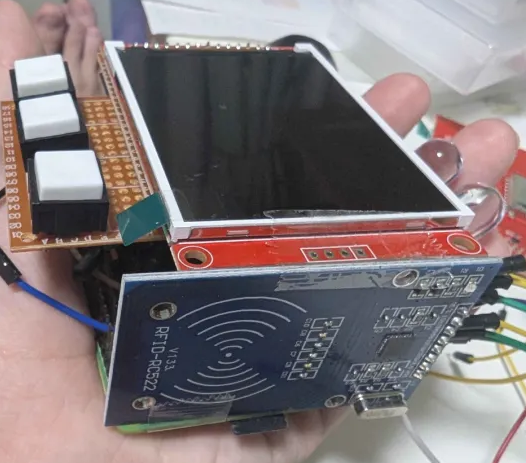
\includegraphics[width=\linewidth]{module.png}};
      \begin{scope}[x={(img.south east)}, y={(img.north west)},
          lbl/.style={fill=navy, text=white, rounded corners=5pt, inner sep=5pt,
            font=\fontsize{16pt}{19pt}\selectfont\bfseries},
          pt/.style={-{Circle[length=10pt]}, line width=3pt, color=navy}]
        \node[lbl] (l1) at (0.17,0.95) {ボタン};
        \draw[pt] (l1.south) -- (0.12,0.80);
        \node[lbl] (l2) at (0.62,0.92) {液晶};
        \draw[pt] (l2.south) -- (0.58,0.72);
        \node[lbl] (l3) at (0.30,0.10) {NFC};
        \draw[pt] (l3.north) -- (0.38,0.30);
      \end{scope}
    \end{tikzpicture}\\[3pt]
    \capt{試作したモジュール}
  \end{minipage}\hfill
  \begin{minipage}[t]{0.32\linewidth}\vspace{0pt}
    \centering
    \photo{lcd_lock.png}{\linewidth}{0.65\linewidth}{}\\[6pt]
    \capt{使用中は他の人を拒否}
    \vspace{10pt}
    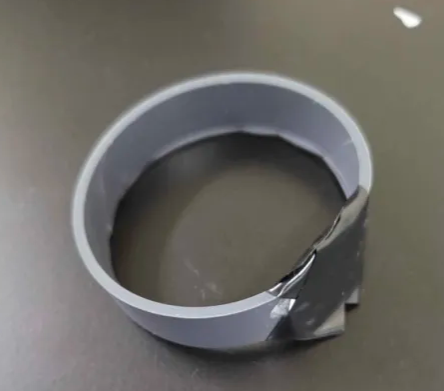
\includegraphics[height=2.6cm]{watchdevice.png}\\[3pt]
    \capt{腕輪型タグ（社員証の代わり）}
  \end{minipage}\hfill
  \begin{minipage}[t]{0.32\linewidth}\vspace{0pt}
    {\fontsize{21pt}{26pt}\selectfont
    \begin{tabular}{@{}>{\bfseries\color{navy}}l@{\hspace{10pt}}l@{}}
      端末 & Raspberry Pi 4 \\
      読取 & NFC (RC522) \\
      表示 & 2.8 型液晶 \\
      入力 & ボタン 3 個 \\
      通信 & MQTT \\
      AI   & Python \\
      音声 & Whisper \\
      LLM  & Gemma 3 \\
    \end{tabular}\par}
  \end{minipage}
}

\block{\bt{現場での使い方}}{%
  \newcommand{\step}[3]{% 番号, 画面, 1 行
    \begin{minipage}[t]{0.235\linewidth}\vspace{0pt}\centering
      {\color{blue}\bfseries\fontsize{30pt}{30pt}\selectfont #1}\\[8pt]
      \photo{#2}{\linewidth}{0.75\linewidth}{}\\[6pt]
      {\fontsize{21pt}{27pt}\selectfont\bfseries #3\par}
    \end{minipage}}
  \step{1}{step1_menu.png}{腕輪をかざす}\hfill
  \step{2}{step2_task.png}{AI の提案を承認}\hfill
  \step{3}{step3_guide.png}{急ぐ仕事へ誘導}\hfill
  \step{4}{step4_done.png}{かざして完了}\par
  \vspace{6pt}
  \capt{モジュールの実際の画面（テストモードの仮想モジュールで撮影）}
  \vspace{14pt}
  \begin{minipage}[c]{0.62\linewidth}
    \fcolorbox{ink2!40}{white}{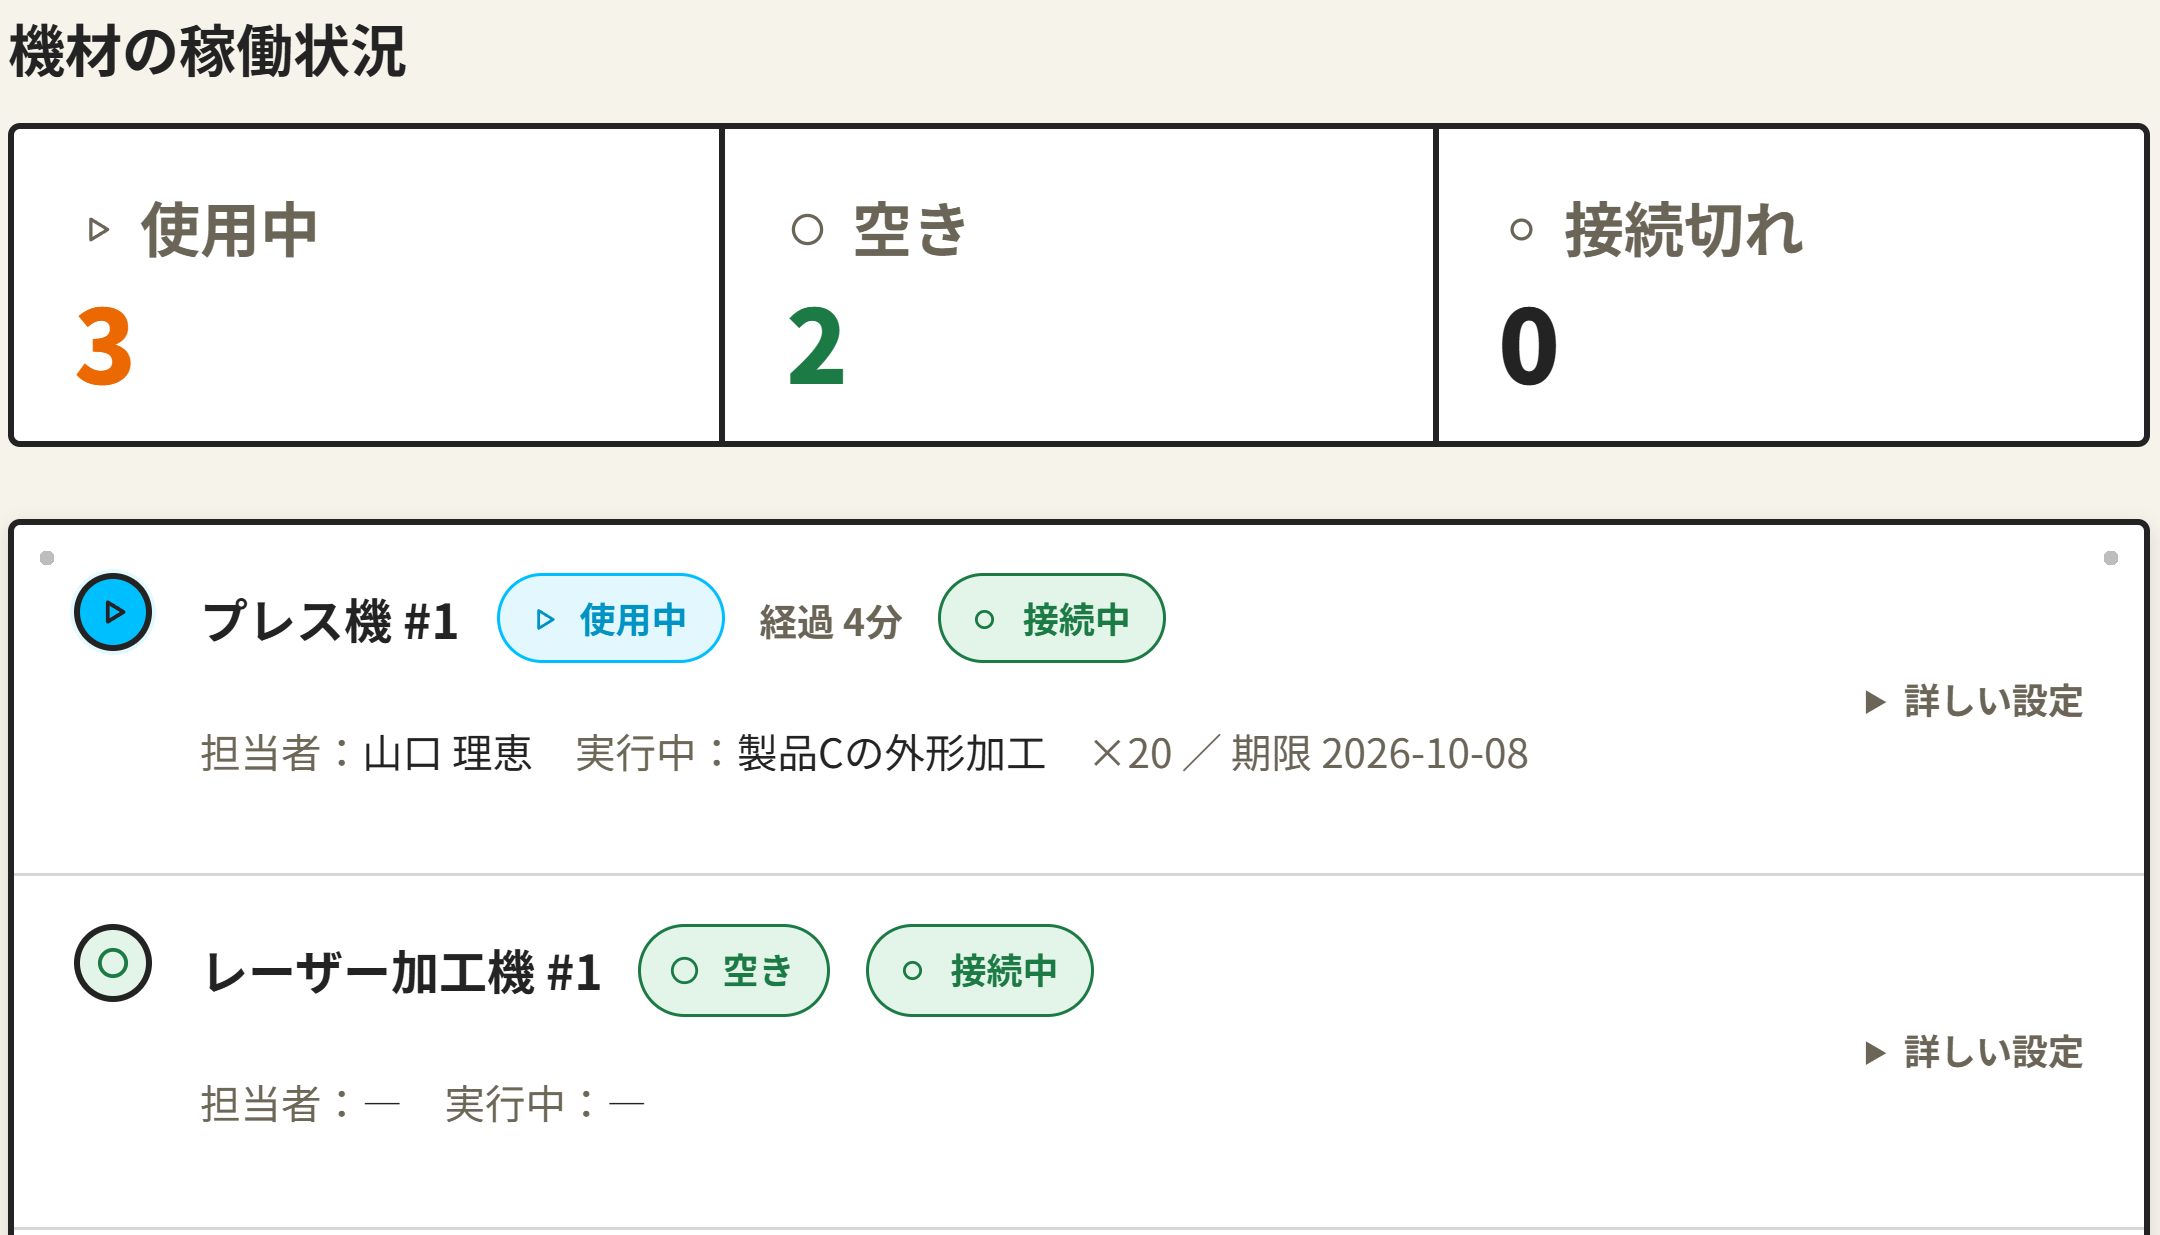
\includegraphics[width=0.97\linewidth]{img/admin_dashboard.png}}\\[4pt]
    \capt{管理画面：機材の稼働状況}
  \end{minipage}\hfill
  \begin{minipage}[c]{0.35\linewidth}
    \head{管理画面}
    \begin{itemize}\fontsize{21pt}{28pt}\selectfont
      \item 使用中・空きが一目で
      \item 誰が何をしているか
      \item 画面は自動で更新
    
    \end{itemize}
    



  \end{minipage}
}

% ================================================================ 右列
\column{0.5}

\block{\bt{使う人のメリット}}{%
  \begin{minipage}[t]{0.488\linewidth}\vspace{0pt}
    \coloredbox[bgcolor=goodtint, fgcolor=ink, framecolor=goodtint, roundedcorners=8, linewidth=0pt]{%
      {\centering{\fontsize{32pt}{38pt}\selectfont\bfseries\color{good}従業員}\par}
      \vspace{14pt}
      \merit{腕輪をかざすだけ}{カードを出さず、PC・スマホ操作もなし}
      \merit{仕事を探さなくてよい}{かざすと次の仕事が出る}
      \merit{完了報告がいらない}{時間は自動で記録}
      \merit{機材の取り合いがない}{使用中は画面に表示}
      \merit{新人にもチャンス}{AIが試しに任せる}
      \merit{声で仕事を登録}{ボタンを押して話すだけ}
    }
  \end{minipage}\hfill
  \begin{minipage}[t]{0.488\linewidth}\vspace{0pt}
    \coloredbox[bgcolor=skytint, fgcolor=ink, framecolor=skytint, roundedcorners=8, linewidth=0pt]{%
      {\centering{\fontsize{32pt}{38pt}\selectfont\bfseries\color{blue}管理者}\par}
      \vspace{14pt}
      \merit{現場が一目で分かる}{誰が・どこで・何を}
      \merit{割り振りは AI}{ボタン 1 つで担当者決定}
      \merit{得意・不得意が分かる}{作業ログから自動で収集}
      \merit{仕事の偏りを防ぐ}{手持ちの多い人を避ける}
      \merit{安全を守る}{無資格者に危険作業なし}
      \merit{IT 担当者が不要}{ブラウザだけで管理、運営}
    }
  \end{minipage}
}

\block{\bt{AI の仕組み}}{%
  \head{割当 AI：実績から「誰に任せるか」を学ぶ}
  {\centering
  \begin{tikzpicture}[font=\fontsize{17pt}{22pt}\selectfont]
    \tikzset{c/.style={text width=5.75cm, minimum height=3.6cm}}
    \newcommand{\st}[2]{{\color{blue}\bfseries\fontsize{26pt}{26pt}\selectfont #1}\ \ {\bfseries\fontsize{21pt}{26pt}\selectfont #2}\\[6pt]}
    \node[box, c] (a) {\st{1}{記録}所要時間\\本人の体感};
    \node[aibox, c, right=9mm of a] (b) {\st{2}{学習}人ごとの速さ\\＋\hl{自信の幅}};
    \node[aibox, c, right=9mm of b] (c) {\st{3}{選択}幅の中から\\くじを引く};
    \node[aibox, c, right=9mm of c] (d) {\st{4}{調整}手持ちで割る\\無資格者を除外};
    \foreach \i/\j in {a/b,b/c,c/d} \draw[arr] (\i) -- (\j);
    \draw[arr, rounded corners=12pt] (d.south) -- ++(0,-0.9) -| (a.south);
  \end{tikzpicture}\par}
  \vspace{10pt}
  \begin{minipage}[c]{0.46\linewidth}
    \begin{tikzpicture}
      \begin{axis}[gem, width=\linewidth, height=0.50\linewidth,
          xlabel={予想される速さ}, ylabel={確からしさ},
          xmin=0, xmax=2.2, ymin=0, ymax=5.6, ytick=\empty, xtick=\empty,
          samples=140, domain=0:2.2, clip=false]
        \addplot[color=navy, fill=navy, fill opacity=0.12]
          {exp(-(x-1.2)^2/(2*0.08^2))/(0.08*sqrt(2*pi))} \closedcycle;
        \addplot[color=orange, fill=orange, fill opacity=0.12]
          {exp(-(x-0.95)^2/(2*0.35^2))/(0.35*sqrt(2*pi))} \closedcycle;
        \draw[navy, line width=3pt, dashed] (axis cs:1.17,0) -- (axis cs:1.17,4.9);
        \draw[orange, line width=3pt, dashed] (axis cs:1.55,0) -- (axis cs:1.55,1.3);
        \node[lab, anchor=east, text=navy, align=right] at (axis cs:1.08,4.4)
          {ベテラン\\幅が狭い};
        \node[lab, anchor=west, text=orange, align=left] at (axis cs:1.42,2.4)
          {新人\\幅が広い};
      \end{axis}
    \end{tikzpicture}
    \capt{破線：くじで引いた値。大きい人に任せる}
  \end{minipage}\hfill
  \begin{minipage}[c]{0.51\linewidth}
    \begin{itemize}\bl
      \item \hl{ベイズ線形回帰}：人ごとに速さを学習
      \item \hl{Thompson Sampling}：くじで選ぶ
      \item 新人にも機会 → 隠れた得意を発見
      \item 手持ちで割る → \hl{全体が早く終わる}
      \item 資格のない作業は\hl{候補から除外}
    \end{itemize}
  \end{minipage}
  \vspace{9pt}

  % ---- 割当の根拠（実際の管理画面）
  \head{AI が選んだ理由（実際の管理画面）}
  \begin{minipage}[c]{0.70\linewidth}
    \fcolorbox{ink2!40}{white}{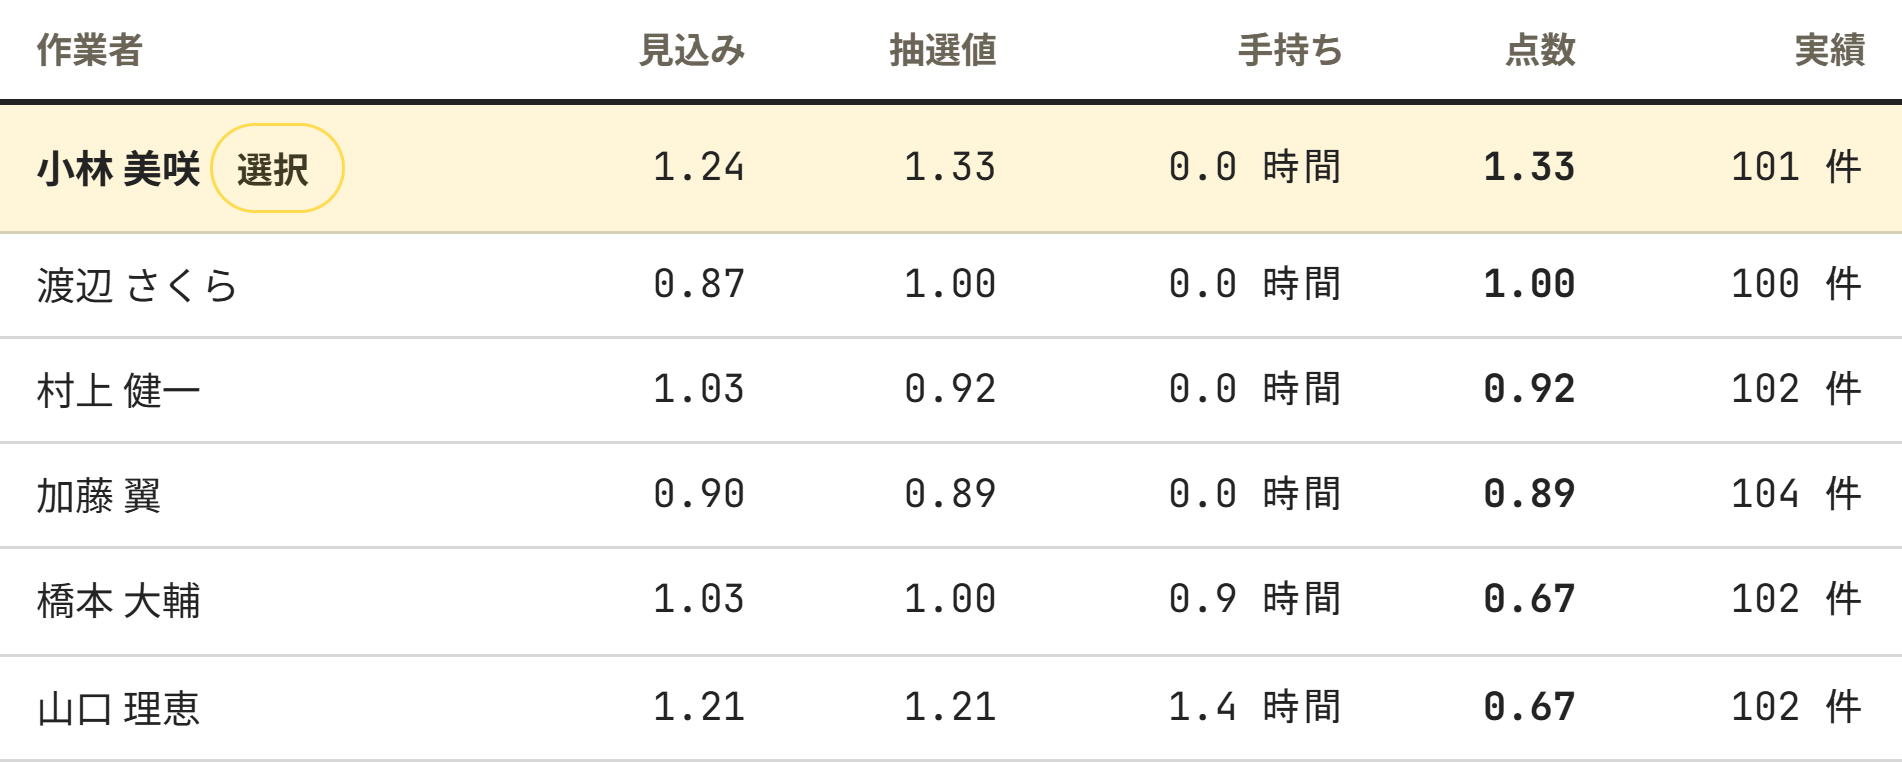
\includegraphics[width=0.97\linewidth]{img/admin_ai_why.png}}\\[4pt]
    \capt{「製品F プレス抜き」の割当。実績 611 件（デモデータ）から学習}
  \end{minipage}\hfill
  \begin{minipage}[c]{0.28\linewidth}
    \raggedright\begin{itemize}\fontsize{20pt}{27pt}\selectfont
      \item 山口さんは\\\hl{手持ち 1.4 時間}
      \\→ 点数 0.67 に
      \item 手の空いた\\\hl{小林さん}を選択
    \end{itemize}
  \end{minipage}
  \vspace{9pt}

  % ---- 効果（シミュレーション）
  \begin{minipage}[c]{0.62\linewidth}
    \head{全員が終わるまでの時間}
    \begin{tikzpicture}
      \begin{axis}[gem, xbar, width=0.78\linewidth, height=0.44\linewidth,
          bar width=18pt, xmin=0, xmax=78, xtick=\empty, axis x line=none,
          ymin=0.4, ymax=4.6, ytick={1,...,4}, y dir=reverse,
          major y tick style={draw=none},
          yticklabels={経験年数順,ランダム,順番に回す,\textbf{Gemmba}},
          nodes near coords={\pgfmathprintnumber[fixed,precision=1,assume math mode=true]{\pgfplotspointmeta}\,分},
          nodes near coords align={horizontal},
          every node near coord/.append style={font=\fontsize{17pt}{17pt}\selectfont\bfseries, color=ink}]
        \addplot[fill=ink2!45, draw=none, bar shift=0pt] coordinates {(63.7,1) (44.4,2) (34.7,3)};
        \addplot[fill=blue, draw=none, bar shift=0pt] coordinates {(25.4,4)};
      \end{axis}
    \end{tikzpicture}
  \end{minipage}\hfill
  \begin{minipage}[c]{0.35\linewidth}
    {\centering
    {\fontsize{46pt}{46pt}\selectfont\bfseries\color{blue}−60\%}\\[4pt]
    {\fontsize{16pt}{20pt}\selectfont\color{ink2}経験年数順と比べて}\\[12pt]
    {\fontsize{46pt}{46pt}\selectfont\bfseries\color{blue}−27\%}\\[4pt]
    {\fontsize{16pt}{20pt}\selectfont\color{ink2}順番に回す割当と比べて}\par}
  \end{minipage}\par
  \capt{シミュレーション：作業者 6 名・150 回 × 20 試行の平均}
  \vspace{10pt}

  \head{音声 AI：話すだけでタスクを登録}
  {\centering
  \begin{tikzpicture}[font=\fontsize{17pt}{22pt}\selectfont]
    \tikzset{c/.style={text width=5.75cm, minimum height=3.2cm}}
    \node[box, c] (v1) {{\bfseries 話す}\\[4pt]{\sm\color{ink2}ボタンを押して}};
    \node[ybox, c, right=9mm of v1] (v2) {{\bfseries 文字にする}\\[4pt]Whisper};
    \node[ybox, c, right=9mm of v2] (v3) {{\bfseries 意味を読む}\\[4pt]Gemma 3（LLM）};
    \node[box, c, right=9mm of v3] (v4) {{\bfseries 検査して登録}\\[4pt]{\sm\color{ink2}資格の漏れを防ぐ}};
    \foreach \i/\j in {v1/v2,v2/v3,v3/v4} \draw[arr] (\i) -- (\j);
  \end{tikzpicture}\par}
  \vspace{10pt}
  {\fontsize{18pt}{23pt}\selectfont
  \renewcommand{\arraystretch}{1.3}
  \begin{tabular*}{\linewidth}{@{\extracolsep{\stretch{1}}}l l c c c@{}}
    \hline
    話した言葉 & タスク名 & 重要度 & 数量 & 期限 \\
    \hline
    「旋盤の切粉清掃を至急お願いします」 & 旋盤の切粉清掃 & \textcolor{red!70!black}{\textbf{至急}} & 1 & -- \\
    「製品 C の外形加工を 20 個、明日まで…」 & 製品Cの外形加工 & \textbf{高} & 20 & 翌日 \\
    \hline
  \end{tabular*}\par}
  \capt{仮想モジュールから送った言葉と、Gemma 3 が実際に作ったタスク}
  \vspace{6pt}
  \begin{itemize}\bl
    \item \hl{すべて現場の PC 内で処理}：工場の情報を外に出さない
  \end{itemize}
}

\end{columns}

% ---------------------------------------------------------------- ユースケース（全幅）
\block{\bt{ユースケース}}{%
  % 1 行：場面（太字）と、そのときの操作の流れ
  \newcommand{\ucrow}[2]{%
    \begin{minipage}[t]{0.27\linewidth}{\bfseries\fontsize{21pt}{26pt}\selectfont #1}\end{minipage}\hfill
    \begin{minipage}[t]{0.72\linewidth}{\fontsize{19pt}{26pt}\selectfont #2}\end{minipage}\par
    \vspace{6pt}}
  \newcommand{\ucbox}[4]{% 地の色, 文字色, 見出し, 行
    \begin{minipage}[t]{0.488\linewidth}\vspace{0pt}
      \coloredbox[bgcolor=#1, fgcolor=ink, framecolor=#1, roundedcorners=8, linewidth=0pt]{%
        {\fontsize{28pt}{34pt}\selectfont\bfseries\color{#2}#3}\par
        \vspace{6pt}
        \def\ucto{\ \textcolor{#2}{→}\ }#4}
    \end{minipage}}
  \ucbox{goodtint}{good}{従業員：}{%
    \ucrow{仕事をする}{腕輪をかざす\ucto 提案を承認\ucto 終わったら再度かざす}
    \ucrow{急ぎの仕事}{かざすと至急の仕事へ誘導\ucto 移動先の画面に通知}
    \ucrow{仕事に気づく}{ボタンを押して話す\ucto AI がタスクとして登録}}\hfill
  \ucbox{skytint}{blue}{管理者：}{%
    \ucrow{仕事を割り振る}{タスクを登録\ucto 「AI 割当」を押す\ucto 担当者が決まる}
    \ucrow{現場を確かめる}{管理画面で、機材の使用中・空きと誰が何をしているかを確認}
    \ucrow{人を育てる}{作業ログから得意・不得意を把握。新人にも AI が試しに任せる}}
}

\end{document}
